\subsection{Limitation}
\label{app:limitation}
Our work is not without limitations. First, while \Bench{} covers three representative benchmarks (ALFWorld, GAIA, and WebShop), it remains limited in scale and domain diversity; extending to multimodal environments, longer-horizon tasks, or safety-critical applications (e.g., healthcare, finance) is an important direction for future work. Second, collecting sufficient data to train a dedicated debugging model would be prohibitively expensive in low-resource academic settings, given the costs of large-scale human annotation. To mitigate this, we instead designed a cost-efficient workflow that leverages prompt engineering with existing LLMs, though this approach may still fall short of the performance achievable with a fully trained, specialized model.


\clearpage
\subsection{\AET{}}
\label{app:aet}
\begin{figure}[htbp]
    \centering
    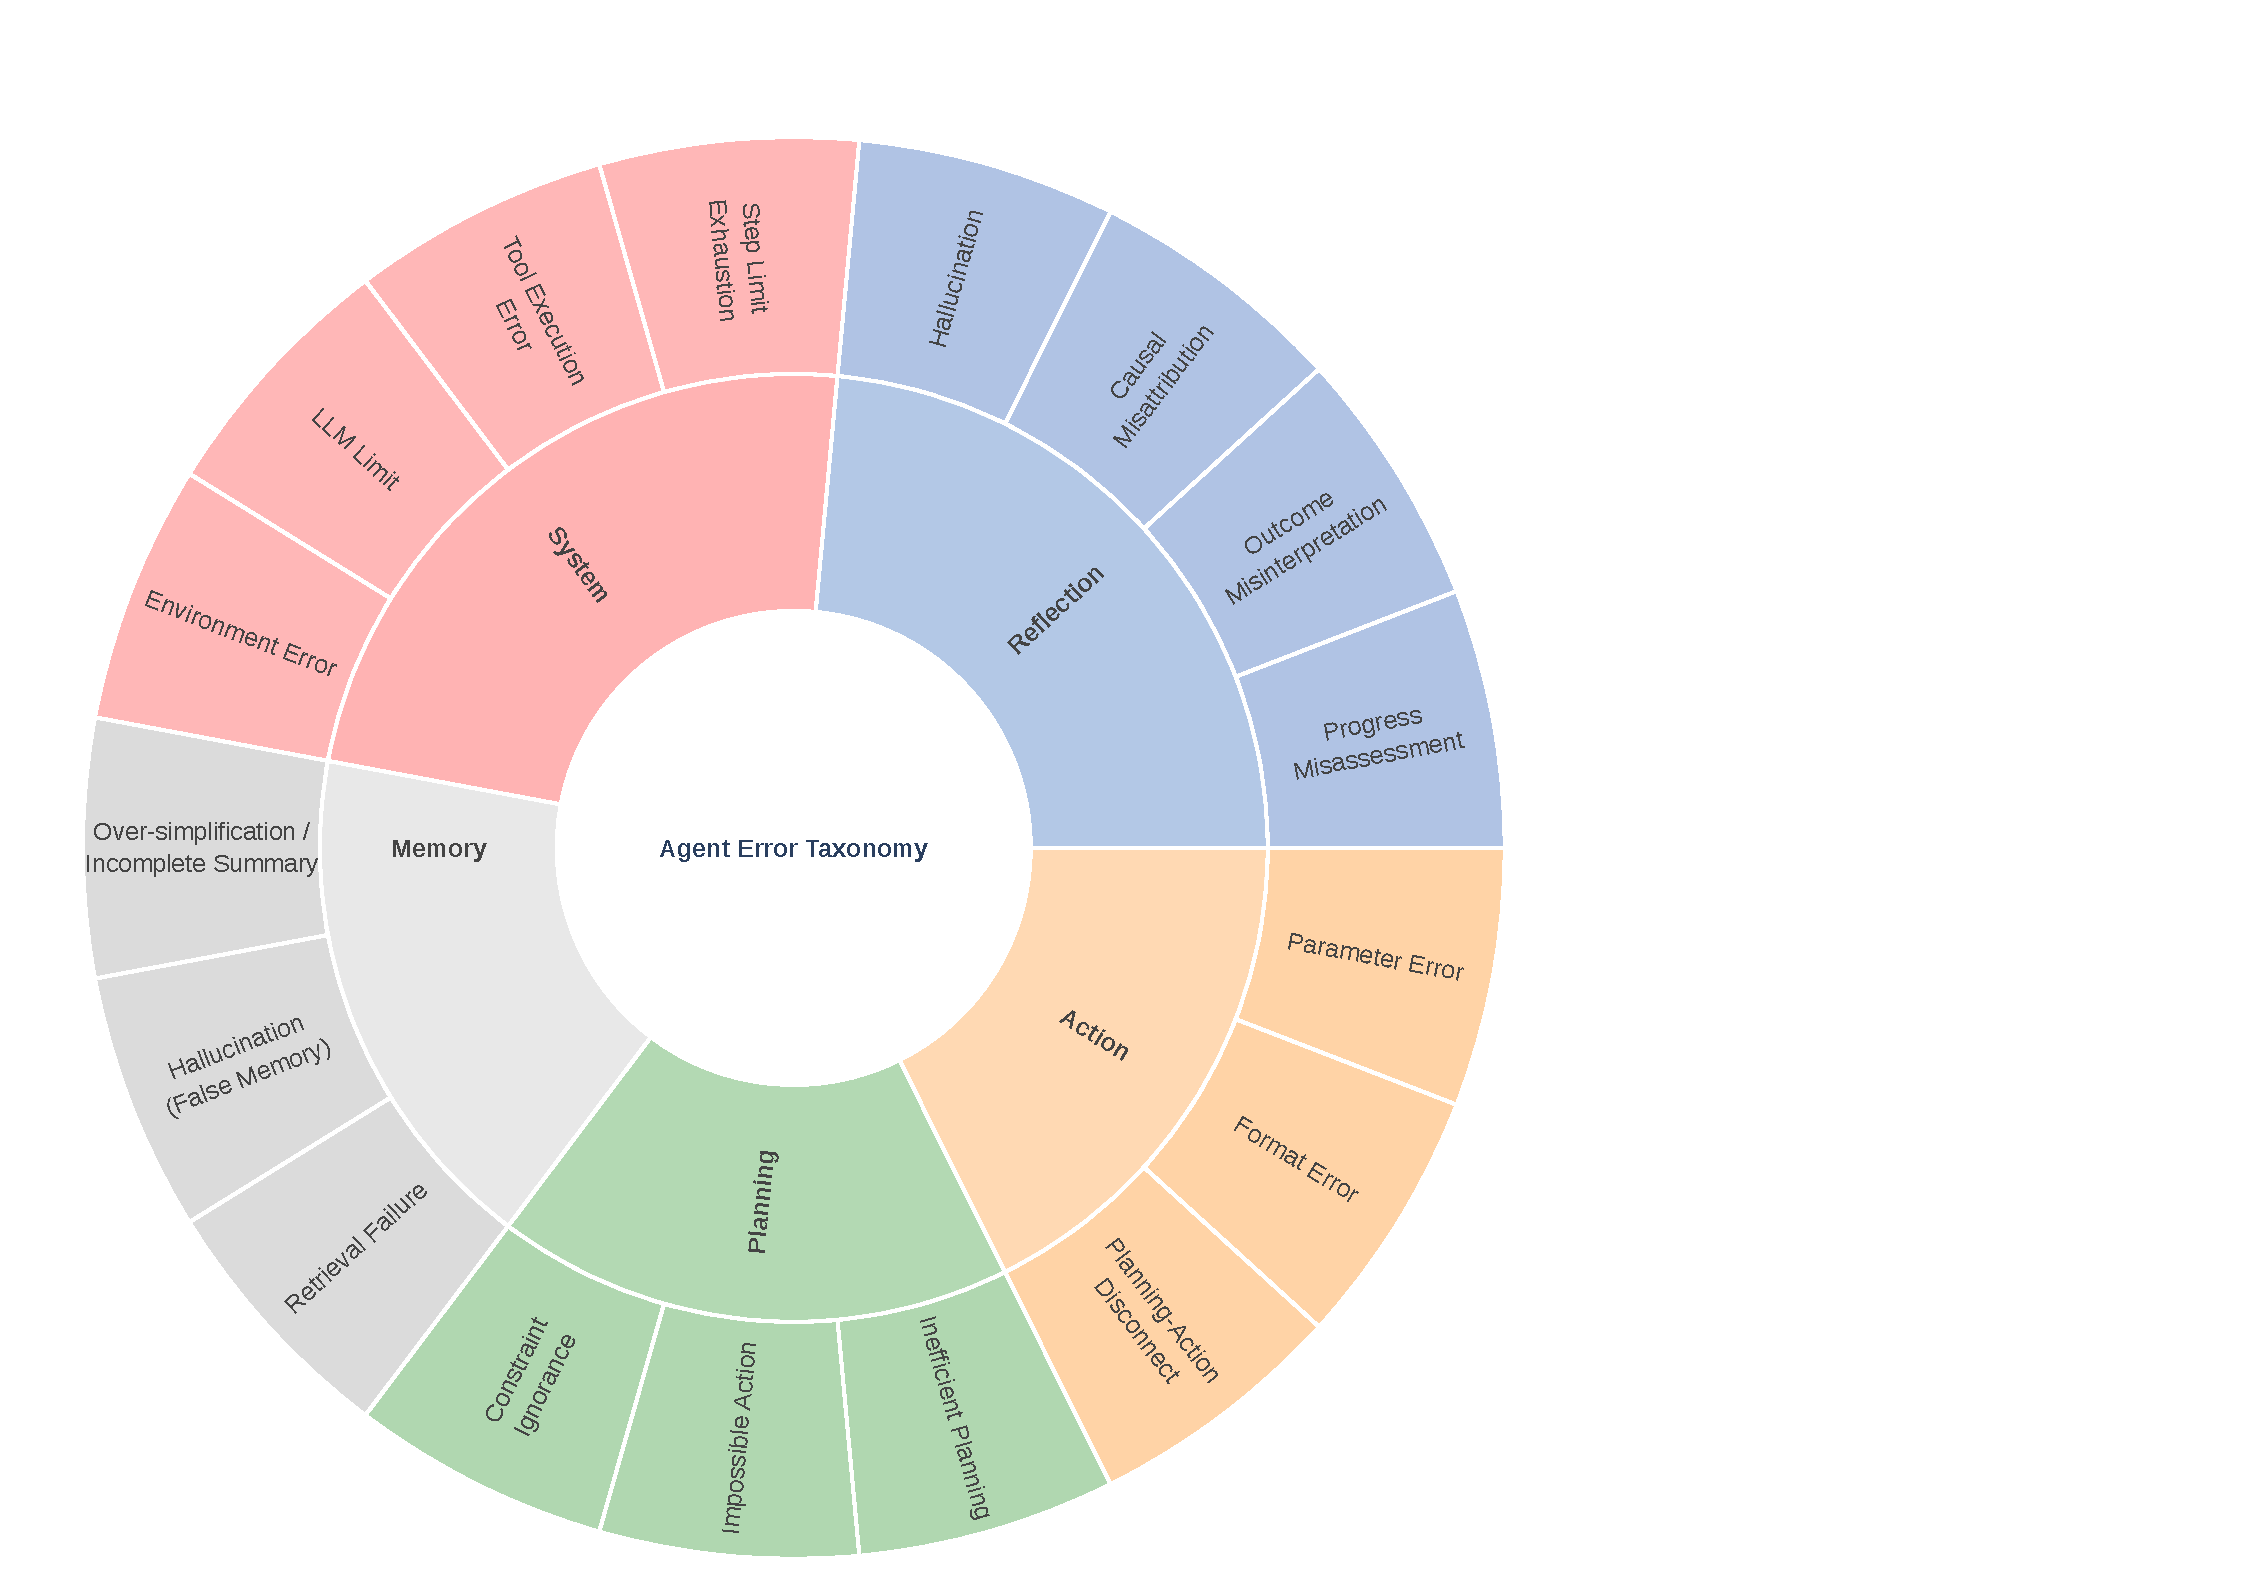
\includegraphics[width=0.7\linewidth]{iclr2026/figures/agent_error_sunburst.pdf}
    \caption{\textbf{Error Taxonomy across all modules}: The hierarchical taxonomy organizes agent errors into five core modules—\emph{Planning}, \emph{Action}, \emph{Reflection}, \emph{Memory}, and \emph{System}. Each outer ring category specifies representative error types, such as constraint ignorance or inefficient planning (Planning), parameter or format errors (Action), causal misattribution or outcome misinterpretation (Reflection), oversimplification or false memory (Memory), and tool execution or environment errors (System). This taxonomy provides a holistic view of where and how failures emerge within modular LLM agents.}

    \label{fig:error_taxnomy}
\end{figure}
\renewcommand{\arraystretch}{1.3} % comfy line height
\setlength{\tabcolsep}{3pt}      % cell padding

\begin{table}[htbp]
\centering
\small
\begin{tabular}{p{0.16\linewidth} p{0.28\linewidth} p{0.50\linewidth}}
\toprule
\rowcolor{gray!15}
\textbf{Module} & \textbf{Error Type} & \textbf{Definition / Explanation} \\
\midrule

% --- Memory ---
\rowcolor{orange!10}Memory   & Over-simplification / Incomplete Summary & Summarizes past info too crudely, ignoring details; leads to flawed reasoning. \\
\rowcolor{orange!10}Memory   & Hallucination (False Memory)             & Recalls events or states that never happened, filling missing gaps with fabricated info. \\
\rowcolor{orange!10}Memory   & Retrieval Failure                         & Relevant info exists but is not retrieved when needed. \\
\hline
% --- Reflection ---
\rowcolor{blue!10} Reflection & Progress Misassessment     & Incorrectly evaluates progress (too optimistic, too pessimistic, or misses completion). \\
\rowcolor{blue!10} Reflection & Outcome Misinterpretation  & Executes an action but misreads the immediate result or environment feedback. \\
\rowcolor{blue!10} Reflection & Causal Misattribution      & Correctly notes failure but blames the wrong cause, misguiding subsequent plans. \\
\rowcolor{blue!10} Reflection & Hallucination              & Reflects on events/results that never occurred. \\
\hline
% --- Planning ---
\rowcolor{green!10}Planning & Constraint Ignorance   & Ignores limits (time, budget, space, etc.) when forming plans. \\
\rowcolor{green!10}Planning & Impossible Action      & Plans a step that is physically/logically impossible given current preconditions. \\
\rowcolor{green!10}Planning & Inefficient Planning   & Plan is overly long or illogical; wastes steps and risks hitting limits. \\
\hline
% --- Action ---
\rowcolor{yellow!15}Action & Planning--Action Disconnect & Chosen actions do not align with the stated plan intent. \\
\rowcolor{yellow!15}Action & Format Error                & Produces syntactically invalid actions. \\
\rowcolor{yellow!15}Action & Parameter Error             & Generates unreasonable or malformed parameters. \\
\hline
% --- System ---
\rowcolor{red!15}System & Step Limit Exhaustion  & Fails due to reaching the maximum step cap despite reasonable behavior. \\
\rowcolor{red!15}System & Tool Execution Error   & External tool/API misbehaves or errors, causing downstream failures. \\
\rowcolor{red!15}System & LLM Limit              & Fails due to API/model constraints (e.g., timeouts, token limits). \\
\rowcolor{red!15}System & Environment Error      & Simulator/environment breaks expected rules (bug/crash/network), not agent’s fault. \\

\bottomrule
\end{tabular}
\caption{\AET{} Definitions}
\end{table}


\clearpage

\subsection{AgentDebug Example}
\begin{figure}[htbp]
    \centering
    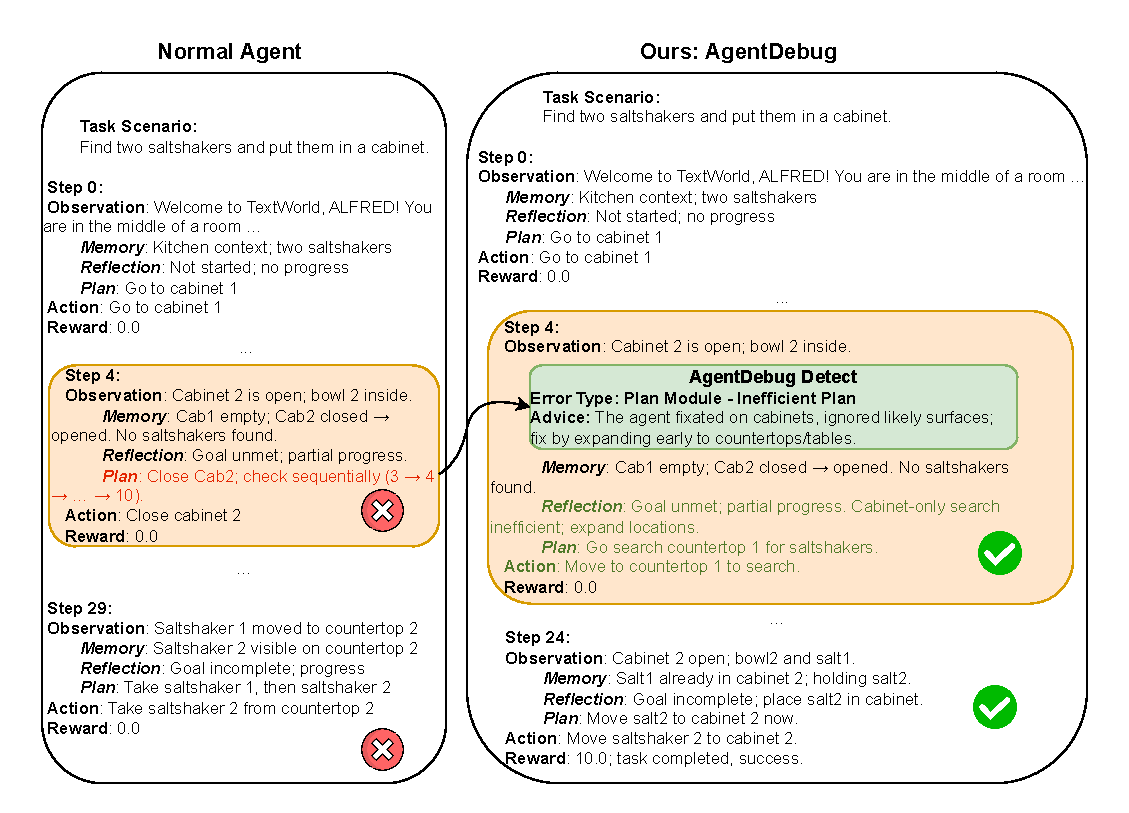
\includegraphics[width=1\linewidth]{iclr2026/figures/AgentDebug_example.pdf}
    \caption{\textbf{AgentDebug example on ALFWorld:} Comparison between a normal agent (left) and our method AgentDebug (right). AgentDebug successfully pinpoints the critical error in the \emph{Plan} module (inefficient cabinet-only search) and provides actionable feedback (expand to countertops/tables). This guidance allows the agent to recover from failure and complete the task successfully.}


    \label{fig:error_taxnomy}
\end{figure}
\clearpage
\subsection{Failure Analysis Across Representative LLMs Agent Benchmarks}
\label{app:failure_analysis}

\begin{figure}[htbp]
    \centering
    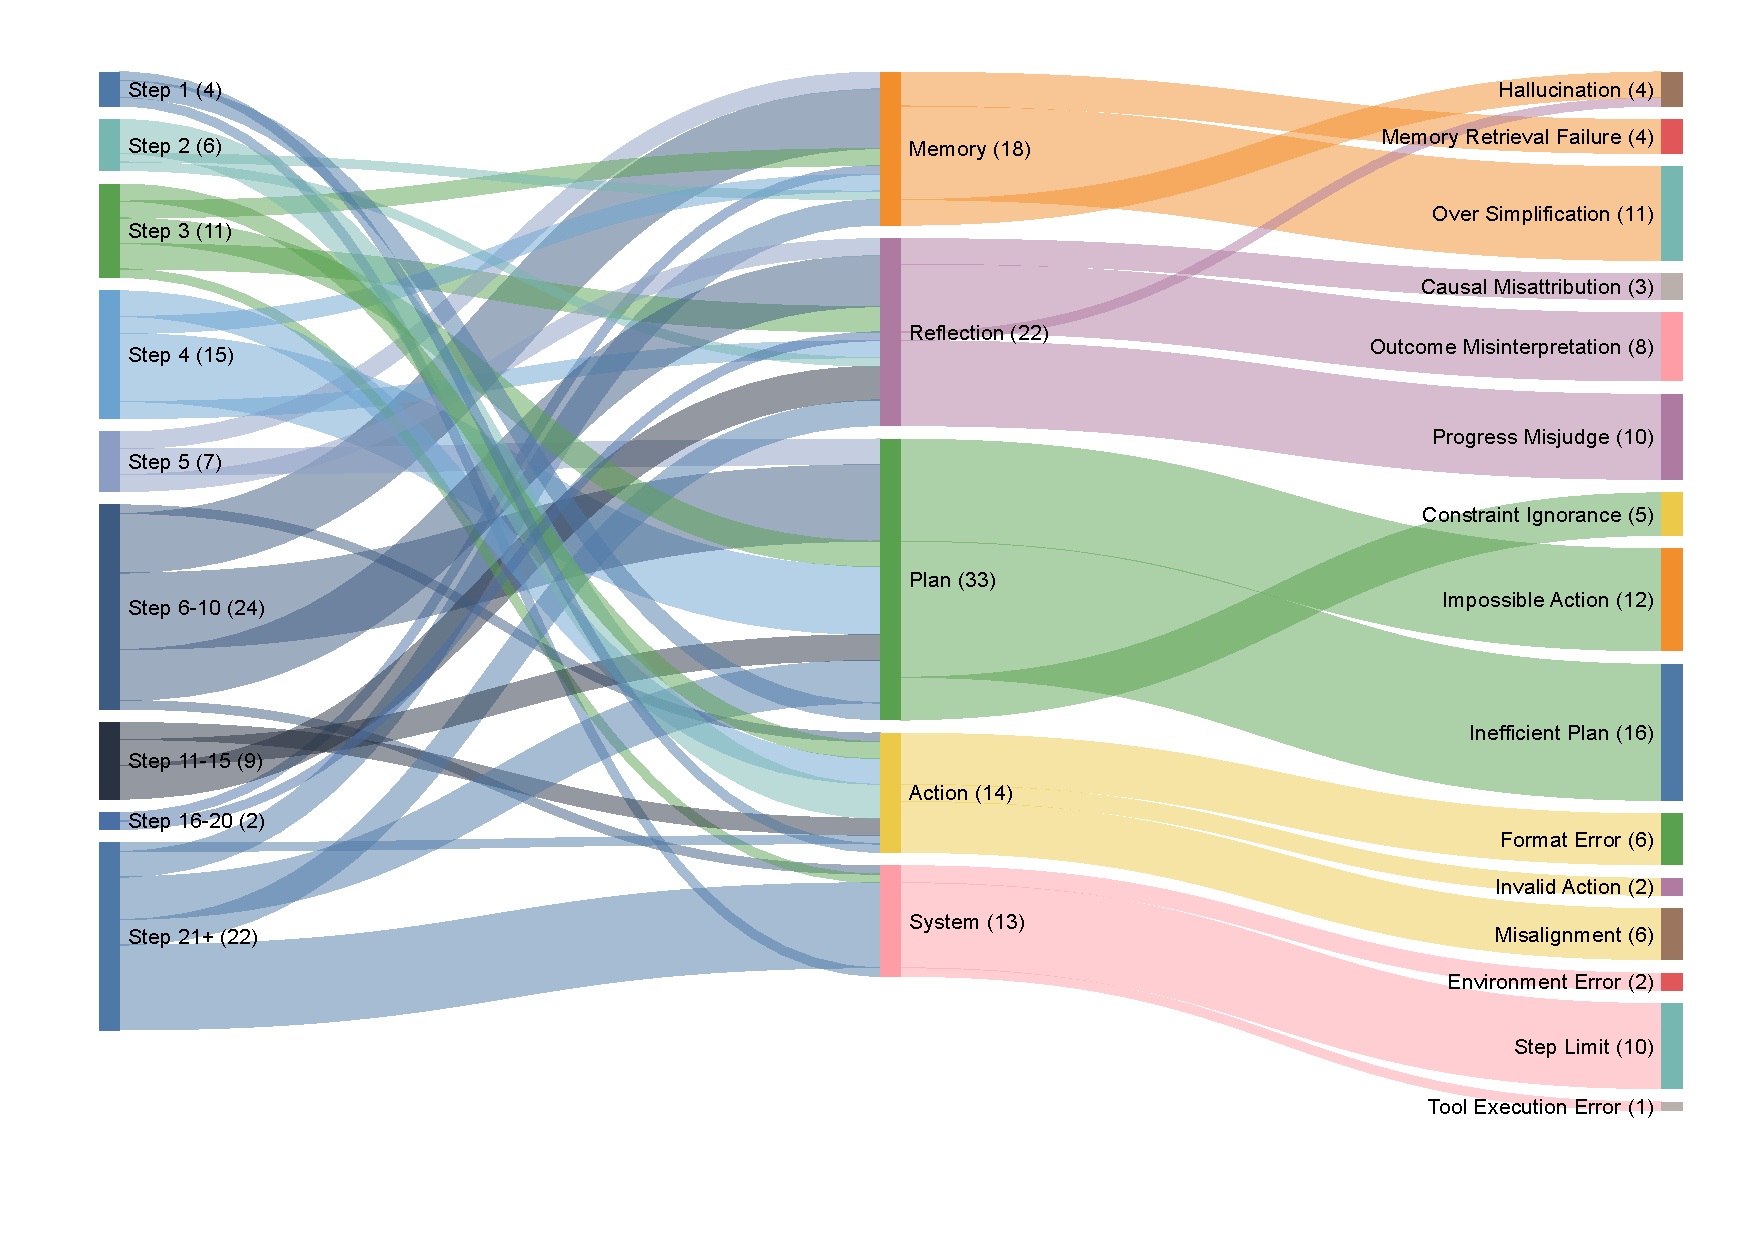
\includegraphics[width=0.8\linewidth]{iclr2026/figures/AlfWorld_Sankey.pdf}
    \caption{Distribution of failure cases in LLM agents on the Alfworld benchmark.}
    \label{fig:failure_analysis}
\end{figure}

\begin{figure}[htbp]
    \centering
    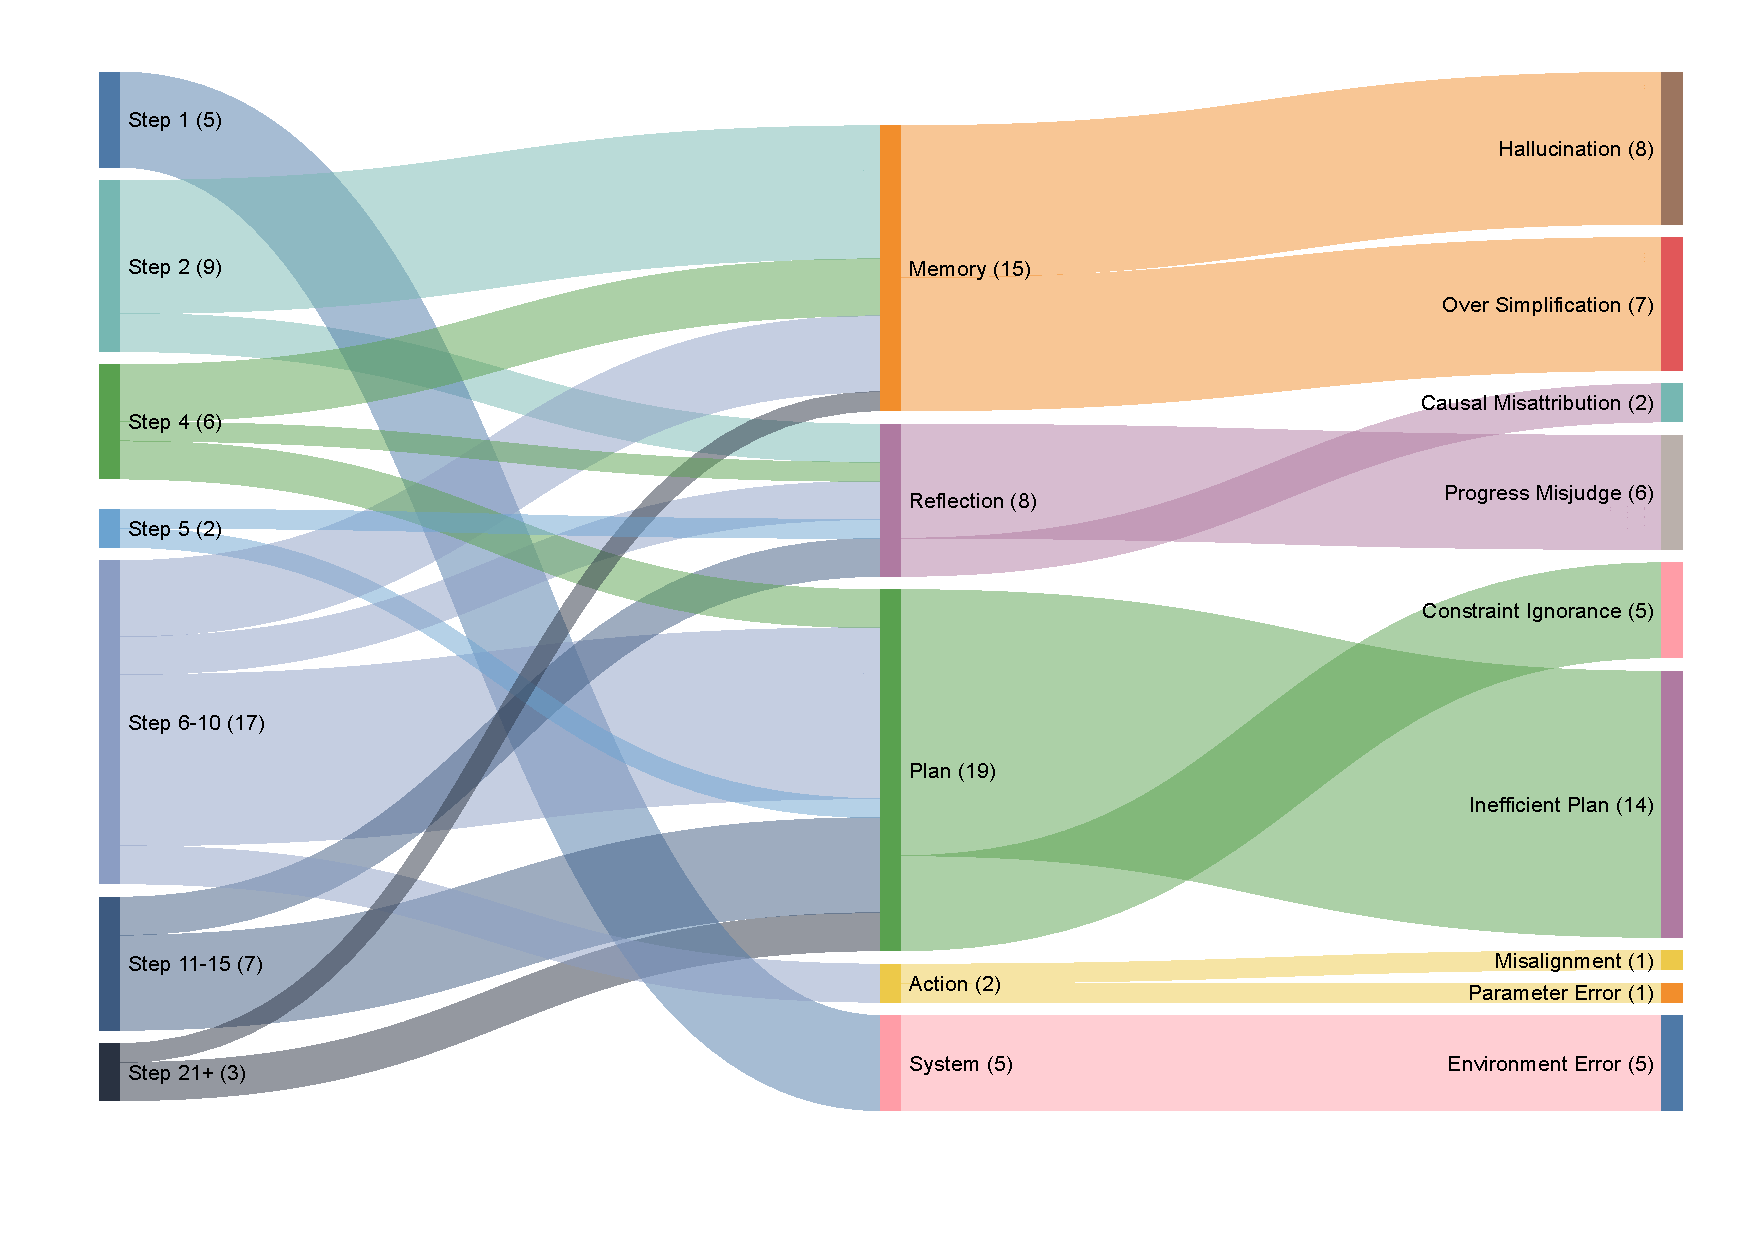
\includegraphics[width=0.8\linewidth]{iclr2026/figures/WebShop_Sankey.pdf}
    \caption{Distribution of failure cases in LLM agents on the Webshop benchmark.}
    \label{fig:failure_analysis}
\end{figure}

\begin{figure}[htbp]
    \centering
    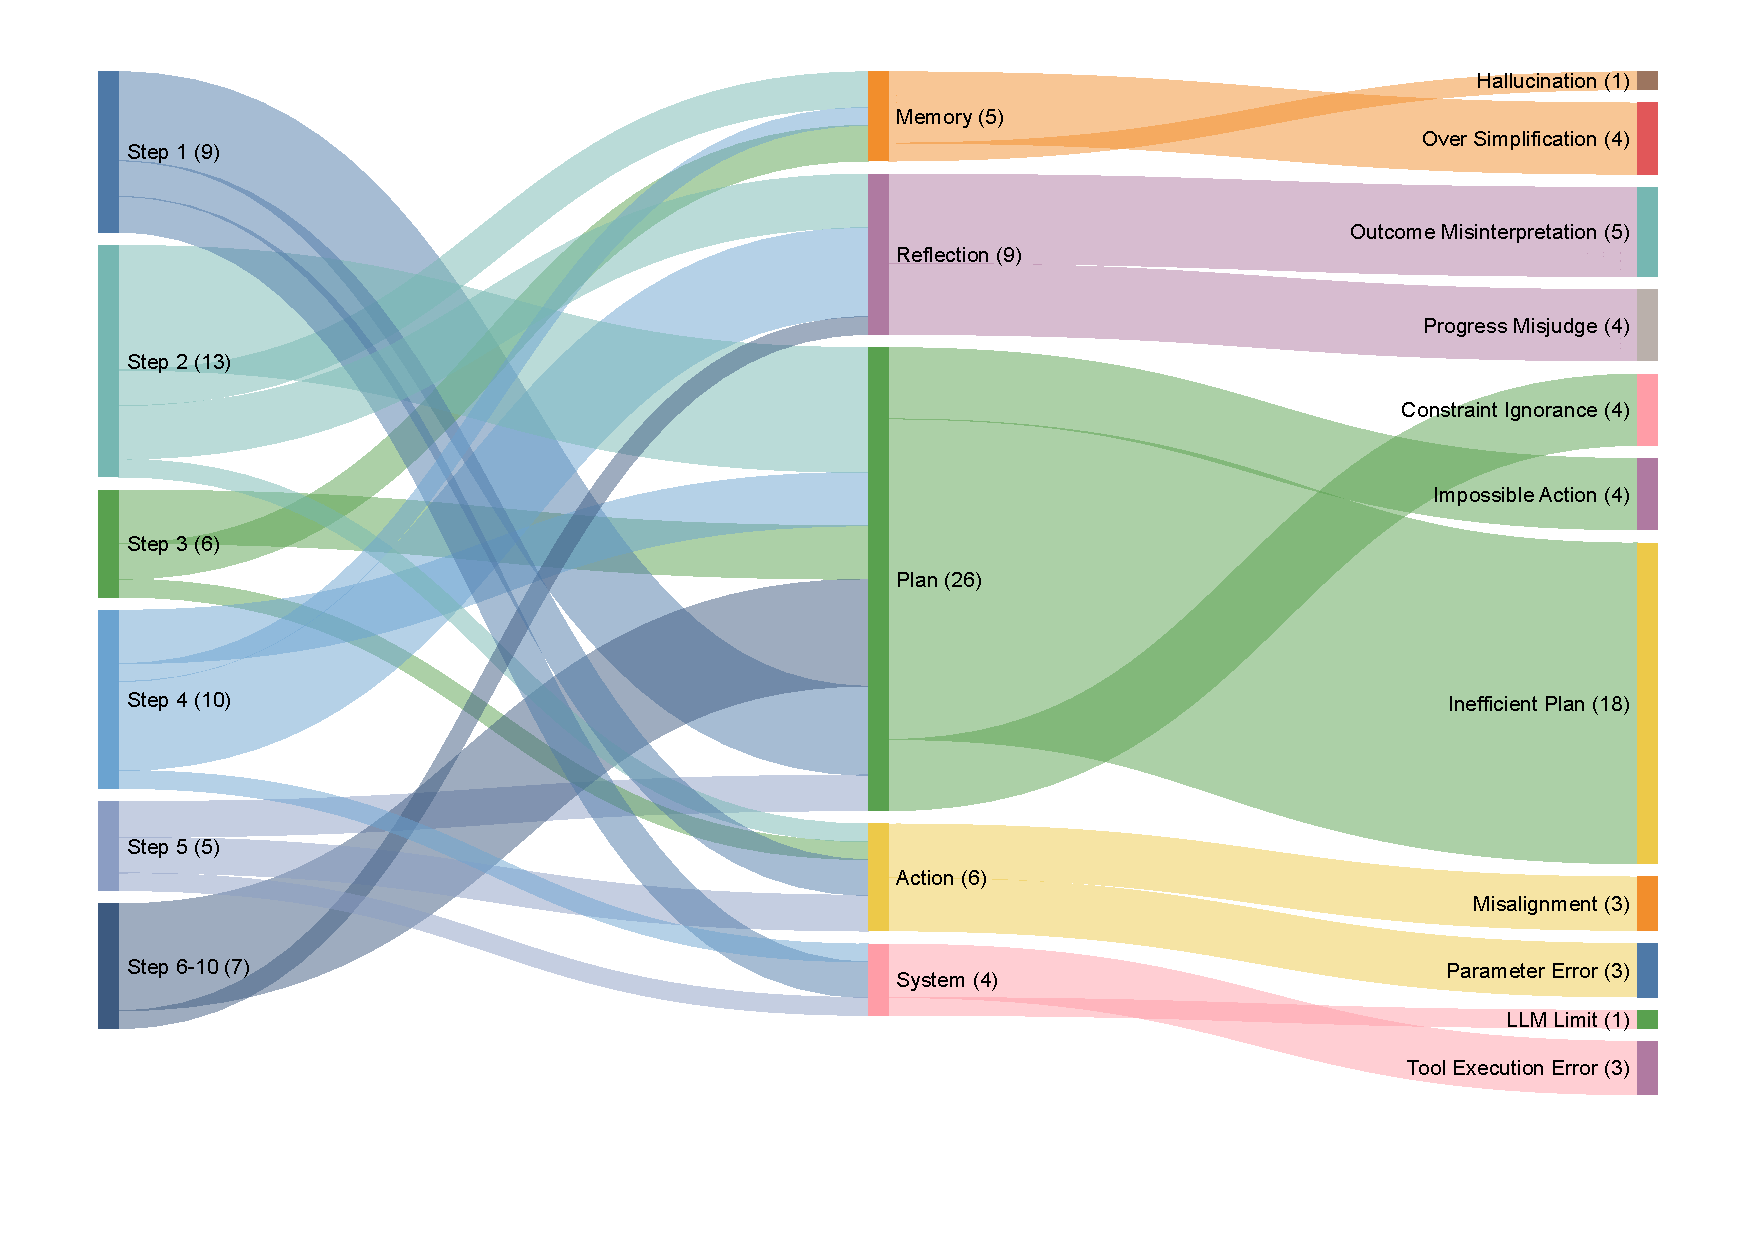
\includegraphics[width=0.8\linewidth]{iclr2026/figures/GAIA_Sankey.pdf}
    \caption{Distribution of failure cases in LLM agents on the GAIA benchmark.}
    \label{fig:failure_analysis}
\end{figure}

\clearpage

\subsection{Prompt}
\label{app:prompt}


\begin{figure*}[htbp]
\centering
\begin{tcolorbox}[
    title=\textbf{Detector Prompt},
    colback=green!1!white,
    colframe=green!50!black,
    fonttitle=\bfseries
]
\small

\small

\textbf{Prompt Overview:}  
Detect whether a specific module output (Memory, Reflection, Planning, Action, or System) contains a defined error, and justify the decision with evidence and reasoning.

\vspace{2mm}

\textbf{Prompt Content (Verbatim):}
\begin{verbatim}
You are an expert at detecting errors in agent trajectories.

TASK: {task_description}
ENVIRONMENT: {environment}
CURRENT STEP: {step_num}

INPUT AND CONTEXT:
{context}

MODULE TO ANALYZE: {module_name}
MODULE OUTPUT (What the agent produced for this module):
{module_content if module_content else "No content found for this 
module"}

ENVIRONMENT RESPONSE AFTER THIS STEP:
{env_response if env_response else "No response"}

{error_definitions}

Based on the SPECIFIC error definitions provided above:
1. Identify if there is an error in this module by checking if the 
output 
matches any error definition
2. If yes, specify which exact error type based on the definitions
3. Provide evidence from the content that directly relates to the 
definition
4. Explain your reasoning showing how it matches the specific 
definition criteria

SPECIAL RULES:
- The "Current Step Input" contains the full user message including 
  conversation history
- Evaluation criteria for each module:
  * Memory: Should correctly summarize/recall from the current step
    input only
  * Reflection: Should correctly reflect based on current input + this 
    step's Memory output
  * Planning: Should plan reasonably based on current input + this 
    step's Memory & Reflection outputs
  * Action: Should execute correctly based on current input + this 
    step's Planning output
- Each module builds on previous modules' outputs FROM THE SAME STEP
- System errors (step_limit, tool_execution_error, etc.) should be 
  identified separately

REQUIRED OUTPUT FORMAT (JSON):
{
    "error_detected": true/false,
    "error_type": "specific_error_type or no_error",
    "evidence": "Quote or description from module content supporting 
    the detection",
    "reasoning": "Explanation of why this is (or isn't) an error based 
     on the definition"
}

Be precise and base your detection on the actual content and error
definitions.
\end{verbatim}
\end{tcolorbox}
\vspace{-1em}
\caption{\textbf{Detector Prompt} used to identify specific error types with evidence and reasoning, returning a strict JSON schema.}
\label{fig:detector_prompt}
\end{figure*}




% \begin{figure*}[htbp]
% \centering
% % 在 tcolorbox 中启用 enhanced jigsaw、breakable、listing engine=verbatim，并将 breaklines=true
% \begin{tcolorbox}[
%     title=\textbf{Planning Evaluation Prompt},
%     colback=blue!1!white,
%     colframe=blue!50!black,
%     fonttitle=\bfseries,
%     % enhanced jigsaw,
%     % breakable,
%     % listing engine=verbatim,
%     % listing options={breaklines=true}
% ]
% \small

% \textbf{Prompt Overview:}  
% This prompt is used to evaluate the \emph{planning} aspect in a multiagent system. 
% It checks whether task assignments, role definitions, workload distribution, 
% and strategic coordination are effectively handled across multiple iterations.

% \vspace{2mm}

% \textbf{Prompt Content (Verbatim):}
% \begin{verbatim}
% Agent Profiles: {agent_profiles}


% \end{verbatim}
% \end{tcolorbox}

% \caption{\textbf{Planning Prompt} used to evaluate how well the agents define roles, assign tasks, and distribute workloads in a multiagent system, with automatic line wrapping.}
% \label{fig:planning_prompt}
% \end{figure*}

\begin{figure*}[htbp]
\centering
\vspace{-8mm}
\begin{tcolorbox}[
    title=\textbf{AgentDebug Prompt},
    colback=blue!1!white,
    colframe=blue!50!black,
    fonttitle=\bfseries,
    % enhanced jigsaw,
    % breakable,
    % listing engine=verbatim,
    % listing options={breaklines=true}
]
\small

\textbf{Prompt Overview:}  
Identify the earliest root-cause error that made success impossible and provide iterative follow-up guidance. Produces a structured JSON report of the critical step, module, error type, evidence, root cause, and cascading effects.

\vspace{2mm}

\textbf{Prompt Content (Verbatim):}
\begin{verbatim}
You are an expert at identifying critical failure points in agent 
trajectories and providing high-priority, iterative follow-up 
instructions that MUST be followed across all subsequent steps.\n
TASK: {task_description}\nTASK RESULT: FAILED\n\n
DEBUG ITERATION CONTEXT:
- Current debug attempt index: {attempt_index}
- Previously issued follow-up instructions:\n
STEP-BY-STEP ERROR ANALYSIS:\n{all_steps}\n
ERROR DEFINITIONS:\n{error_reference}\n\n
Your job is to identify the CRITICAL ERROR - the earliest and most 
important error that led to task failure, and produce an iterative 
follow-up instruction that will help avoid similar mistakes in future 
attempts.\n\n
CRITICAL ERROR IDENTIFICATION APPROACH:\n You must take a HOLISTIC, 
GLOBAL perspective to identify the true root cause of failure. 
Do NOT rely on any predetermined severity weights or rankings\n
ANALYSIS GUIDELINES:
1. Consider the ENTIRE trajectory from a global perspective - understand 
the task goal and how the agent's path diverged from success
2. Find the EARLIEST point where the agent made a decision or error that 
set it on an irreversible path to failure
3. Early exploration steps (steps 1-3) are often normal and should NOT 
be marked as critical unless there's a clear, fundamental error
4. An error is critical if:
   - It represents the ROOT CAUSE that made task success impossible
   - It caused a cascade of subsequent errors
   - The trajectory could have succeeded if THIS specific error had 
   not occurred
   - IMPORTANT: Correcting this specific error would fundamentally 
   change the trajectory toward success
5. Focus on causal chains - trace backwards from the failure to find 
the origin point
6. IMPORTANT: Step 1 only has planning and action modules - no 
memory or reflection is possible at step 1 since there's no history yet
   - Do NOT mark step 1 memory/reflection as critical errors
   - Early steps without memory/reflection modules are expected
7. Consider System and Others categories as potential critical errors:
   - System errors (step_limit, tool_execution_error, llm_limit, 
   environment_error) may also be the true cause of failure
   - For example, if the agent was performing correctly but hit 
   step_limit, that IS the critical error
   - Others category captures unusual failures not covered by standard 
   error types\n
Identify the TRUE ROOT CAUSE that made the task unrecoverable.\n
REQUIRED OUTPUT FORMAT (JSON):\n{
    "critical_step": <step_number>,
    "critical_module": "<module_name: memory|reflection|planning|action|
    system|others>",
    "error_type": "<specific_error_type_from_definitions>",
    "root_cause": "Concise description of the fundamental problem",
    "evidence": "Specific quote or observation from trajectory 
    supporting this identification",
    "correction_guidance": "Actionable advice for the agent to avoid the 
    same mistake in that step",
    "cascading_effects": [{ "step": <step_number>, 
    "impact": "description" }]}
\end{verbatim}
\end{tcolorbox}
\vspace{-1em}
\caption{\textbf{AgentDebug Prompt} used to locate the root cause of task failure and issue structured correction guidance.}
\label{fig:agentdebug_prompt}
\end{figure*}




% \begin{figure*}[htbp]
% \centering
% \begin{tcolorbox}[
%     title=\textbf{KPI Evaluation Prompt},
%     colback=yellow!1!white,
%     colframe=yellow!50!black,
%     fonttitle=\bfseries
% ]
% \small

% \textbf{Prompt Overview:}  
% This prompt is used for Key Performance Indicator (KPI) assessment within a multiagent research task, determining whether specific milestones (like “form 5q” or “improve 5q”) have been achieved in each iteration.

% \vspace{2mm}

% \textbf{Prompt Content (Verbatim):}
% \begin{verbatim}
% [Context]
% **Task:**

% \end{verbatim}
% \end{tcolorbox}

% \caption{\textbf{KPI Prompt} used to check if milestones such as “form 5q” or “improve 5q” have been achieved in a research iteration.}
% \label{fig:kpi_prompt}
% \end{figure*}



\begin{figure*}[htbp]
\centering
\vspace{-8mm}
\begin{tcolorbox}[
    title=\textbf{Baseline Prompts},
    colback=yellow!1!white,
    colframe=yellow!50!black,
    fonttitle=\bfseries
]
\small

\textbf{Prompt Overview:}  
Prompts used as baselines, including Tree-of-Thought (ToT) value scoring and proposal, a vanilla debug template, and a Self-Refine feedback prompt.

\vspace{2mm}

\textbf{Prompt Content (Verbatim):}
\begin{verbatim}
1. Prompts for TOT value prompt
base_prompt = (
    f"You are evaluating candidate NEXT actions for an agent in 
    {self.env_type}.\n"
    f"Rate how promising each action is for achieving the goal from the 
    CURRENT state.\n"
    f"{history_section}Current observation:\n{obs}\n\n"
    f"Candidates (JSON list): {cand_json}\n\n"
    "Scoring rubric (strict):\n"
    "- Use the FULL 0.0–1.0 range. Do NOT give all 1.0 or all equal 
    scores.\n"
    "- 0.9–1.0: Directly and obviously advances the goal with minimal 
    risk.\n"
    "- 0.7–0.9: Strongly promising next step.\n"
    "- 0.4–0.7: Plausible but uncertain; depends on missing 
    preconditions.\n"
    "- 0.2–0.4: Weak progress or likely redundant.\n"
    "- 0.0–0.2: Invalid, circular, or contradicts recent 
    history/admissible options.\n"
    "- Penalize repeating the same action that just failed, no-ops, 
    or irrelevant moves.\n"
    "Return ONLY a JSON array of floats, aligned to input order, length 
    equals number of candidates.")
Propose prompt: prompt = (
    f"You are choosing the agent's next action in {env_type}.\n"
    f"{history_desc}Current observation:\n{obs}\n\n"
    f"Propose up to {k} different, concrete next actions the agent 
    could take next.\n"
    f"Each proposal must be a single executable action string in the 
    exact format expected by the environment.\n"
    f"Avoid repeating ineffective or redundant actions from the 
    history above.\n"
    f"Return only a JSON list of strings, no extra 
    text.{diversity_desc}")

2. Prompts for vanilla debug
PROMPT_TEMPLATE = ( "Trajectory :\n{trajectory}\n\n"
    "Your task:\n"
    "1. Identify the earliest step whose action, plan, reflection, or 
    memory directly leads the agent off track or repeats ineffective 
    behaviour.\n"
    "2. Reference that exact step number (0-based) as shown in the 
    trajectory. Do not shift to later steps of that error.\n"
    "3. Explain why the chosen step is wrong, citing relevant 
    observation/action details.\n"
    "4. Suggest a concrete alternative for that same step that would 
    move the agent toward success 
    (e.g., a specific action to take instead).\n\n"
    "Respond strictly in the following format (single spaces around 
    colons, no extra text):\n"
    "step: <number>\n"
    "reason: <one concise, specific sentence>\n"
    "suggestion: <one actionable suggestion for that step>\n")

3. Prompts for Self-Refine
PROMPT_TEMPLATE = ( "Current result: {trajectory}\n\n"
    "Why is this trajectory not finished the task?\n\n" "Feedback:")
\end{verbatim}
\end{tcolorbox}
\caption{\textbf{Baseline Prompts.} Includes Tree-of-Thought value and proposal prompts, a vanilla debug template for earliest error localization, and a Self-Refine feedback prompt.}
\label{fig:baseline_prompts}
\end{figure*}




\begin{figure*}[htbp]
\centering
\vspace{-8mm}
% 在 tcolorbox 中启用 enhanced jigsaw、breakable、listing engine=verbatim，并将 breaklines=true
\begin{tcolorbox}[
    title=\textbf{Environment Rollout Prompt - ALFWorld },
    colback=orange!1!white,
    colframe=orange!50!black,
    fonttitle=\bfseries,
    % enhanced jigsaw,
    % breakable,
    % listing engine=verbatim,
    % listing options={breaklines=true}
]
\small

\textbf{Prompt Overview:}  
This is the environment rollout prompt for ALFWorld.

\vspace{2mm}

\textbf{Prompt Content (Verbatim):}
\begin{verbatim}
ALFWORLD_TEMPLATE_NO_HIS = """
You are an expert agent operating in the ALFRED Embodied Environment.
Your task is: {task_description}
Your current observation is: {current_observation}
Your admissible actions of the current situation are: 
{admissible_actions}.\n
Please begin by analyzing the situation and planning your approach:\n
<plan>\n Plan the next step:
- Given what I've learned, what should I do next?
- Please explain why this plan is helpful for the next action?
- What do I expect this action to achieve?\n</plan>\n
<action>\n
Finally, choose ONE admissible action for the current step and choose 
it within {admissible_actions}. \n</action>
"""

ALFWORLD_TEMPLATE = """ You are an expert agent operating in the ALFRED 
Embodied Environment. Your task is to: {task_description} Prior to 
this step, you have already taken {step_count} step(s). Below are 
the most recent {history_length} observaitons and the corresponding 
actions you took: {action_history} You are now at step {current_step} 
and your current observation is:  {current_observation} Your admissible 
actions of the current situation are: {admissible_actions}.\n
Now it's your turn to take an action.\n
You should first recall relevant past experiences and reason from our 
conversation history, then MUST summarize within <memory> </memory> 
tags like this:\n
<memory> \n 
Look at the past observations and actions from our conversation history.
- Please retrieve the most relavent memory for this step including the 
relevant observation and action in a RAG style along with step number.
- These memory shall be helpful milestones to solve this task.</memory>

After that, you should reflect on the last action and its outcome, 
then MUST summarize within <reflection> </reflection> tags like this:

<reflection>
Reflect on the last action and its outcome
- Did I complete the task goal?
- Was last action successful or did it encounter issues?
- Am I making progress toward the task goal?
- If the action did not go as expected and did not result in progress,
provide constructive feedback to guide the next planning step.
</reflection>

After that, you should plan next step based on memory and reflection, 
then MUST summarize within <plan> </plan> tags like this:

<plan>
Plan the next step based on memory and reflection
- Given what I've learned, what should I do next?
- Please explain why this plan is helpful for the next action?
- What do I expect this action to achieve?
</plan>

<action>
Finally, choose ONE admissible action for the current step and choose it 
within {admissible_actions}.
</action>
"""
\end{verbatim}
\end{tcolorbox}
\vspace{-1em}
\caption{\textbf{Environment Rollout Prompt} used for ALFWorld.}
\label{fig:taskscore_prompt}
\end{figure*}




\begin{figure*}[htbp]
\centering
% 在 tcolorbox 中启用 enhanced jigsaw、breakable、listing engine=verbatim，并将 breaklines=true
\begin{tcolorbox}[
    title=\textbf{Environment Rollout Prompt - Webshop },
    colback=orange!1!white,
    colframe=orange!50!black,
    fonttitle=\bfseries,
    % enhanced jigsaw,
    % breakable,
    % listing engine=verbatim,
    % listing options={breaklines=true}
]
\small

\textbf{Prompt Overview:}  
This is the environment rollout prompt for Webshop.

\vspace{2mm}

\textbf{Prompt Content (Verbatim):}
\begin{verbatim}
WEBSHOP_TEMPLATE_NO_HIS = """
You are an expert agent operating in the WebShop e-commerce environment.
Your task is: {task_description}
Your current observation is: {current_observation}
Your admissible actions of the current situation are: 
{available_actions}.\n
Please begin by analyzing the situation and planning your approach:

<plan> Plan the next step:
- Given what I've learned, what should I do next?
- Please explain why this plan is helpful for the next action?
- What do I expect this action to achieve? </plan>

<action> Finally, choose ONE admissible action for the current step and 
choose it within {available_actions}. </action>
"""

WEBSHOP_TEMPLATE = """
You are an expert agent operating in the WebShop e-commerce environment.
Your task is to: {task_description}
Prior to this step, you have already taken {step_count} step(s). Below 
is a compact summary of all steps: {action_history}
You are now at step {current_step} and your current observation is: 
{current_observation}
Your admissible actions of the current situation are: 
{available_actions}.\n Now it's your turn to take an action.

You should first recall relevant past experience and reason from the 
history context, then MUST summarize within <memory> </memory> tags 
like this: <memory> Look at the history context above.
- Please retrieve the most relevant memory for this step including the 
relevant observation and action in a RAG style along with step number.
- These memory should be helpful milestones to solve this task.</memory>

After that, you should reflect on the last action and its outcome, then 
MUST summarize within <reflection> </reflection> tags like this:

<reflection> Reflect on the last action and its outcome
- Did I complete the task goal?
- Was last action successful or did it encounter issues?
- Am I making progress toward the task goal?
- If the action did not go as expected and did not result in progress, 
provide constructive feedback to guide the next planning step. 
</reflection>

After that, you should plan the next step based on memory and 
reflection, then MUST summarize within <plan> </plan> tags like this:

<plan> Plan the next step based on memory and reflection
- Given what I've learned, what should I do next?
- Please explain why this plan is helpful for the next action?
- What do I expect this action to achieve? </plan>

<action> Finally, choose ONE admissible action for the current step and 
choose it within {available_actions}. </action>
"""
\end{verbatim}
\end{tcolorbox}

\caption{\textbf{Environment Rollout Prompt} used for Webshop.}
\label{fig:taskscore_prompt}
\end{figure*}

\begin{figure*}[htbp]
\centering
\vspace{-8mm}
% 在 tcolorbox 中启用 enhanced jigsaw、breakable、listing engine=verbatim，并将 breaklines=true
\begin{tcolorbox}[
    title=\textbf{Environment Rollout Prompt - GAIA },
    colback=orange!1!white,
    colframe=orange!50!black,
    fonttitle=\bfseries,
    % enhanced jigsaw,
    % breakable,
    % listing engine=verbatim,
    % listing options={breaklines=true}
]
\small

\textbf{Prompt Overview:}  
This is the environment rollout prompt for GAIA.

\vspace{2mm}

\textbf{Prompt Content (Verbatim):}
\begin{verbatim}
TOOL_USE_TEMPLATE_NO_HIS = """
You are an expert research assistant capable of using various tools to 
gather information and solve complex problems.\nTask: {task_description}
Available Tools: {available_tools}\n Current Observation: 
{current_observation}\n  Instructions:
1. Analyze the task and determine what information you need
2. Use available tools to gather information when needed
3. Reason through the information step by step  
4. When you have sufficient information, provide your final answer 
in <answer></answer> tags\n Format for tool usage:\n <action> tool: 
[tool_name] parameters: {{"param1": "value1", "param2": "value2"}} 
</action>\n Now it's your turn to take an action. You shall first reason 
step-by-step about the current situation. This reasoning process MUST be 
enclosed within <plan></plan> tags. Once you've finished your reasoning, 
you should either use a tool or provide your final answer within 
<answer> </answer> tags.\n """\n TOOL_USE_TEMPLATE_LAST_STEP = """
You are an expert research assistant capable of using various tools to 
gather information and solve complex problems.\n Task: 
{task_description}\n Prior to this step, you have already taken 
{step_count} step(s). Below are the full {history_length} observations
and the corresponding actions you took: {action_history}\n
You are now at step {current_step} and this is the final step.
Current Observation: {current_observation}
You must provide your final answer within <answer> </answer> tags.
Even if the evidence is incomplete, infer the most plausible answer.
Never respond with "unknown", "cannot determine", or similar phrases."""
TOOL_USE_TEMPLATE = """ You are an expert research assistant capable of 
using various tools to gather information and solve complex problems.\n
Task: {task_description}\n Prior to this step, you have already taken 
{step_count} step(s). Below are the most recent {history_length} 
observations and the corresponding actions you took: {action_history}\n 
You are now at step {current_step}. Current Observation: 
{current_observation}\n Available Tools:{available_tools}\n  You should 
first recall relevant past experiences and reason from our conversation 
history, then MUST summarize within <memory_recall> </memory_recall> 
tags like this: <memory>
Look at the past observations and actions from our conversation history.
- Please retrieve the most relavent memory for this step including the 
relevant observation and action in a RAG style with the step number.
- These memory should be helpful milestones to solve this task.</memory>
After that, you should reflect on the last action and its outcome, then 
MUST summarize within <reflection> </reflection> tags like this:
<reflection> Reflect on the last action and its outcome
- Did I complete the task goal?
- Was last action successful or did it encounter issues?
- Am I making progress toward the task goal?
- If the action did not go as expected and did not result in progress, 
provide feedback to guide the next planning step. </reflection>\n 
Given from the analysis from the memory and reflection, if we 
get the final answer,we should provide it within <answer></answer> tags.
If we don't get the final answer, you should plan the next step based on 
memory and reflection, then MUST summarize within <plan> </plan> tags 
like this: <plan> Plan the next step based on memory and reflection
- Given what I've learned, what should I do next?
- Please explain why this plan is helpful for the next action?
- What do I expect this action to achieve? </plan>\n
Finally, choose ONE admissible action for the current step and present 
it within the <action> </action> tags. <action> action: [tool_name]  
parameters: {{"param1": "value1", "param2": "value2"}}</action> """
\end{verbatim}
\end{tcolorbox}
\vspace{-1em}
\caption{\textbf{Environment Rollout Prompt} used for Webshop.}
\label{fig:taskscore_prompt}
\end{figure*}



% \begin{mybox}{GAIA Planner Prompt}
% \centering
% % 在 tcolorbox 中启用 enhanced jigsaw、breakable、listing engine=verbatim，并将 breaklines=true
% \footnotesize
% \begin{Verbatim}[breaklines=true]
% TASK_ANALYSIS_SYSTEM = """You are an expert multi-agent system architect. Analyze the given task with deep understanding and provide a comprehensive analysis.

% Consider these aspects:
% 1. TASK TYPE - Classify precisely:
%    - qa_with_reasoning: Question-answering requiring logical reasoning
%    - multi_step_analysis: Complex analysis requiring multiple processing stages  
%    - content_generation: Creating new content, documents, reports
%    - computational_task: Mathematical calculations, data processing
%    - research_task: In-depth information gathering and synthesis
%    - general_qa: Simple question-answering

% 2. COMPLEXITY ASSESSMENT:
%    - low: Simple, straightforward tasks requiring 1-2 steps
%    - medium: Moderate complexity requiring 3-5 processing steps
%    - high: Complex tasks requiring 6+ steps, domain expertise, or sophisticated reasoning

% 3. REQUIRED TOOLS - Select from available tools:
%    Available tools: {available_tools}

% 4. AGENT CONFIGURATION - For each required tool, specify:
%    - name: Descriptive agent name (e.g., "WebResearcher", "DataAnalyst", "CodeExecutor")
%    - role: Create meaningful, task-specific roles (e.g., "information_gatherer", "computational_specialist", "data_processor", "final_synthesizer", "document_analyzer", "web_navigator", etc.)
%    - Be creative with roles - they should reflect the agent's specific function in solving the task

%    Example role types you can use as inspiration:
%    * information_gatherer: Searches for and collects relevant information from various sources
%    * computational_specialist: Executes calculations, data processing, and analytical tasks
%    * document_analyzer: Processes and extracts information from documents and files
%    * evidence_synthesizer: Integrates information from multiple sources into coherent conclusions
%    * task_coordinator: Breaks down complex tasks and manages workflow execution
%    * content_creator: Generates reports, summaries, and structured outputs
%    * domain_expert: Provides specialized knowledge in specific fields
%    * data_processor: Handles data transformation, cleaning, and formatting
%    * web_navigator: Specializes in web search and online information retrieval
%    * final_synthesizer: Provides comprehensive final answers and conclusions


% 5. DOMAIN EXPERTISE needed (technology, science, business, finance, healthcare, etc.)

% 6. PROCESSING REQUIREMENTS:
%    - Sequential vs parallel processing needs
%    - Validation/verification requirements
%    - Error handling complexity

% IMPORTANT HARD RULES:
% - The tool 'create_chat_completion' is reserved for the FINAL agent only. Include it exactly once and position it as the LAST step in the workflow. Do NOT assign or call it in intermediate steps or by non-final agents.

% IMPORTANT: Based on the GAIA task level {level}, we recommend using approximately {recommended_agents} agents for optimal performance. However, you can adjust this number based on task complexity:
% - Use fewer agents (1-2) for very simple, single-step tasks
% - Use the recommended number ({recommended_agents}) for typical level {level} tasks  
% - Use more agents (up to {max_agents}) only if the task genuinely requires complex multi-step processing

% You must limit your agent recommendations to a maximum of {max_agents} agents total. Plan efficiently within this constraint.
% Respond with detailed JSON analysis including your reasoning.

% Analyze the task and respond with a JSON object containing:
% {{
%   "task_type": "general_qa|research_task|computational_task|multi_step_analysis",
%   "complexity": "low|medium|high", 
%   "required_tools": ["tool1", "tool2"],
%   "agents": [
%     {{
%       "tool": "tool_name",
%       "name": "AgentName", 
%       "role": "specific_role_based_on_function",

%     }}
%   ],
%   "estimated_steps": number,
%   "domain_areas": ["domain1", "domain2"]
% }}

% Example:
% {{
%   "task_type": "research_task",
%   "complexity": "medium",
%   "required_tools": ["browser_use", "create_chat_completion"],
%   "agents": [
%     {{
%       "tool": "browser_use",
%       "name": "WebResearcher",
%       "role": "academic_information_gatherer", 

%     }},
%     {{
%       "tool": "create_chat_completion",
%       "name": "ReasoningSynthesizer",
%       "role": "evidence_synthesizer",

%     }}
%   ],
%   "estimated_steps": 3,
%   "domain_areas": ["general_knowledge"]
% }}
% """
% \end{Verbatim}

% \label{fig:gaia planner prompt}
% \end{mybox}





% begin{figure*}[htbp]
% \centering
% \begin{tcolorbox}[
%     title=\textbf{Good Communication Case \#1},
%     colback=red!1!white,
%     colframe=red!50!black,
%     fonttitle=\bfseries
% ]
% \small

% \textbf{Case Overview:}  
% In this case, multiple agents repeatedly send the same or very similar messages, and one agent communicates only with itself. These behaviors lead to inefficient or unproductive exchanges that do not significantly advance the task at hand.

% \vspace{2mm}
% \textbf{Conversation (Verbatim):}
% \begin{verbatim}
% Iteration 1:  | Iteration 2: In Session 33132321-4f22-47a9-9e62-e3d5a2429a5e 
% \end{verbatim}

% \end{tcolorbox}
% \caption{\textbf{Good Communication Case \#1.} An example of two research agents dive deep into one potential research topics, and give insightful views.}
% \label{fig:bad_comm_case_1}
% \end{figure*}

% Memory

\clearpage
\subsection{Error Types Examples}

% Memory
\subfile{iclr2026/appendix/error_type/over_simplification}

% Plan
\subfile{iclr2026/appendix/error_type/impossible_action}
\subfile{iclr2026/appendix/error_type/constraint_ignore}
\subfile{iclr2026/appendix/error_type/inefficient_plan}

% Action
\subfile{iclr2026/appendix/error_type/misalignment}
\subfile{iclr2026/appendix/error_type/format_error}

% reflection
\subfile{iclr2026/appendix/error_type/progress_misjudge}